\documentclass[11pt,a4paper]{article}

\usepackage[margin=22mm]{geometry}
\usepackage{times}
\usepackage{amsmath,amssymb}
\usepackage{booktabs}
\usepackage{graphicx}
\usepackage{microtype}
\usepackage[hidelinks]{hyperref}
\usepackage{caption}
\usepackage{setspace}
\setstretch{1.07}
\captionsetup{font=small,skip=4pt}
\graphicspath{{figures/}}

\title{\vspace{-8mm}DASE7506 MP1 Report\\[4pt]
}
\author{%
  Student ID: 3036837930 \quad Name: Shang Zishuai \\
  GitHub: \texttt{zss019/DASE7506-Project-1} \quad Issue \#107
}
\date{Reported full-test FP32 BPB: \textbf{1.48544}\\[2pt]}

\begin{document}
\maketitle
\vspace{-6mm}

\section{Introduction}

The assignment is to train a language model from random initialisation on the supplied WikiText-2 splits and BPE-2048 tokenizer, then minimise \emph{bits per byte} (BPB) on the frozen test split. Evaluation uses independent causal windows of 256 tokens, FP32, and must remain reproducible on CPU. The resource cap is at most five times the baseline's CPU scoring time, 4\,GiB peak evaluation RAM, and 64\,MiB of uncompressed inference assets. The starter GPT (width 128, four layers, four heads, $1.09$M parameters) scores about $2.10$ test BPB.

This report documents one submitted predictor and the evidence required by the guide: a reproduced baseline; a comparison at the same number of processed training targets; an ablation of the mechanisms that actually move BPB; and a critical account of quality--cost trade-offs. All architecture and hyperparameter choices were made on validation. The test split was scored only after a method was frozen.

\section{Method}

\subsection{Model}

The submitted model is a decoder-only Transformer with context length 256 and vocabulary 2048. Relative to the starter classroom GPT the block is:
\begin{itemize}
  \item \textbf{RMSNorm} instead of LayerNorm, and \textbf{no linear biases}.
  \item \textbf{Rotary position embeddings (RoPE)} instead of a learned absolute position table.
  \item A \textbf{GELU MLP} with hidden width $4\times d$, matching the baseline FFN family rather than a gated SwiGLU.
  \item \textbf{Dropout $0.2$} on token embeddings, attention, and residual branches (training only).
  \item \textbf{GPT-2-style residual-output initialisation}, $\sigma=0.02/\sqrt{2L}$.
  \item Tied input and output embeddings (already in the baseline).
\end{itemize}
The submitted size is $d{=}256$, $L{=}8$, 4 heads: \textbf{6\,820\,096} parameters (26.0\,MiB checkpoint).

\subsection{Training}

Training uses the supplied trainer with additional, default-off flags. The submitted run uses CUDA with BF16 autocast and seed 17, which was fixed in advance rather than selected after seeing other seeds. It trains for $7000$ steps at batch $128$ and context $256$, i.e.\ $229\,376\,000$ processed targets ($\approx 63$ epochs of the $3.61$M-token train split). The optimiser is AdamW with $\beta=(0.9,0.999)$, gradient clip $1.0$, peak learning rate $4\times 10^{-3}$, $300$-step warmup, and a cosine floor of $2\%$ of peak. Weight decay is $0.3$ and excludes 1-D parameters (norm gains). An EMA copy with decay $0.9995$ is validated and saved.

\section{Reproduced baseline}

The official recipe (starter classroom GPT, 1\,200 steps, batch 32, seed 17, AdamW LR $10^{-3}$, 100-step warmup, cosine to $10\%$ of peak) was run on CPU with four threads, as in the code README. Table~\ref{tab:baseline} reports the reproduced scores.

\begin{table}[t]
\centering
\caption{Reproduced starter GPT on the official baseline recipe (CPU, four threads, seed 17).}
\label{tab:baseline}
\small
\begin{tabular}{lrrrr}
\toprule
Split & BPB & Token PPL & Parameters & Train tokens \\
\midrule
Validation & 2.0711 & 79.5 & 1\,088\,256 & 9\,830\,400 \\
\textbf{Test (CPU FP32)} & \textbf{2.10126} & 80.8 & same & same \\
\bottomrule
\end{tabular}
\end{table}

This matches the advertised $\approx 2.10$ test BPB. Scoring took $7.5$\,s on the development CPU (Xeon Gold 6248, shared host); peak RSS was $2.11$\,GiB. GPU replays of the \emph{same architecture and token budget} (Section~\ref{sec:matched}) give validation BPB $2.0747\pm 0.0037$ over three seeds, so the CPU/GPU gap is noise.

\section{Matched-token comparison and architecture ablation}
\label{sec:matched}

The guide asks for a comparison at the same number of processed training targets, and an ablation of the key mechanism. One paired sweep covers both.

Keeping $1\,200$ steps $\times$ $32$ $\times$ $256 = 9.83$M targets, seed $\in\{17,18,19\}$, and the baseline optimiser, each architectural switch was turned on or off independently. Table~\ref{tab:matched} and Figure~\ref{fig:matched} summarise validation BPB.

\begin{table}[t]
\centering
\caption{Validation BPB at $9.83$M targets (mean $\pm$ sample SD, three seeds). $\Delta$ is paired against the modern block.}
\label{tab:matched}
\small
\begin{tabular}{lrrr}
\toprule
Config & Params & Val.\ BPB & $\Delta$ vs modern \\
\midrule
Classroom GPT & 1\,088\,256 & $2.0747\pm 0.0037$ & $+0.237$ \\
\textbf{Modern (RMSNorm+RoPE+SwiGLU, no bias, scaled init)} & 1\,049\,216 & $1.8379\pm 0.0021$ & $0$ \\
RoPE $\to$ learned positions & 1\,081\,984 & $1.9955\pm 0.0047$ & $+0.158$ \\
SwiGLU $\to$ GELU & 1\,049\,728 & $1.9311\pm 0.0010$ & $+0.093$ \\
No residual scaled init & 1\,049\,216 & $1.8426\pm 0.0022$ & $+0.005$ \\
RMSNorm $\to$ LayerNorm & 1\,050\,368 & $1.8343\pm 0.0002$ & $-0.004$ \\
Add biases & 1\,054\,504 & $1.8353\pm 0.0024$ & $-0.003$ \\
\bottomrule
\end{tabular}
\end{table}

\begin{figure}[t]
\centering
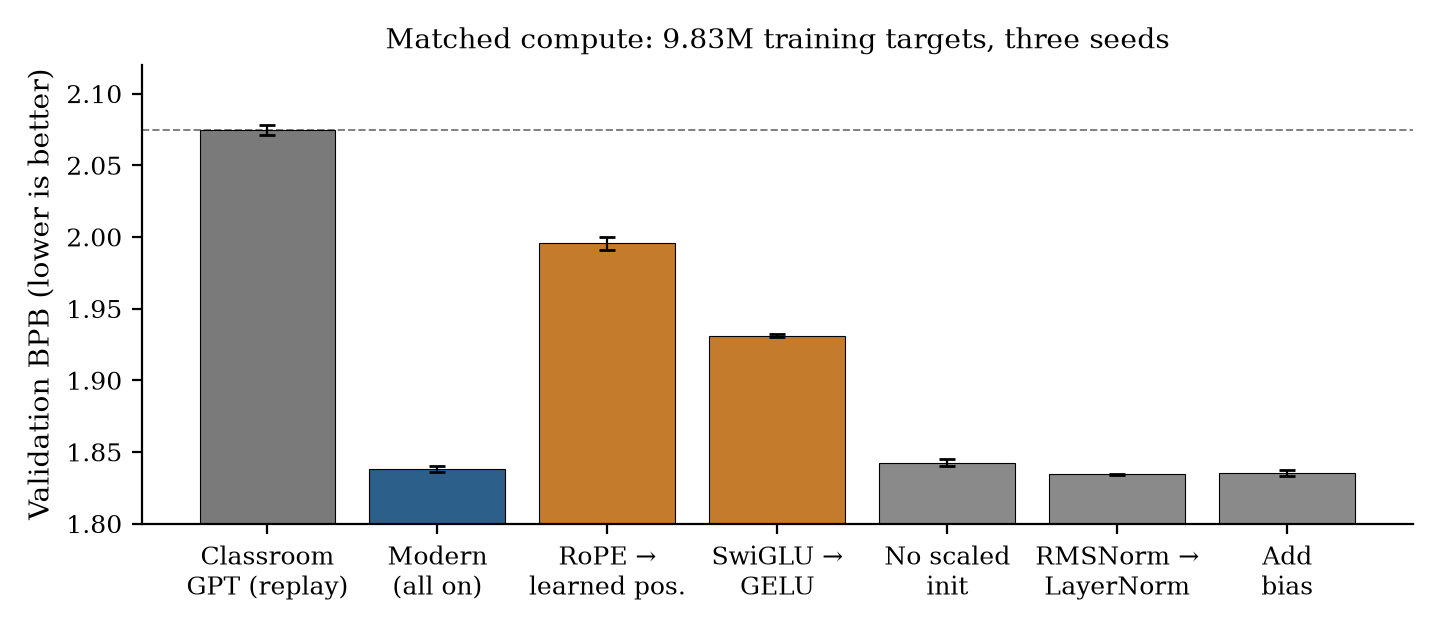
\includegraphics[width=\linewidth]{fig1_matched_ablation.png}
\caption{Matched-token architecture ablation. Error bars are sample standard deviations over seeds 17/18/19. The dashed line is the classroom GPT mean.}
\label{fig:matched}
\end{figure}

Under a \emph{short} pass over a $3.6$M-token corpus, replacing the starter block with a modern block cuts validation BPB by \textbf{0.24}, far larger than seed scatter ($\mathrm{SD}\approx 0.002$--$0.005$). The two mechanisms that explain almost all of that gap are:
\begin{enumerate}
  \item \textbf{RoPE ($\approx 0.16$ BPB).} A learned $256\times d$ position table must be estimated from few unique windows; late positions are rare. RoPE encodes \emph{relative} offset in the attention logits with no extra parameters, which is a better inductive bias when data are scarce.
  \item \textbf{SwiGLU ($\approx 0.09$ BPB).} At matched parameter count (hidden width $8/3\,d$ vs $4d$ GELU), a gated MLP is a more efficient feed-forward nonlinearity---on this \emph{short} schedule.
\end{enumerate}
Scaled residual init is a small, stable gain ($\approx 0.005$, about $3\times$ the paired SD). RMSNorm versus LayerNorm, and removing bias, are \textbf{not} distinguishable from noise at this size; LayerNorm is even slightly better. Those two knobs were therefore treated as optional modern defaults, not as claimed contributions.

CPU scoring of the modern $1.05$M model was $7.2$\,s versus $6.4$\,s for the baseline on the same host: RoPE adds a rotation, but the ratio is $\approx 1.1\times$, far inside the $5\times$ cap.

\section{Scaling and regularisation}

WikiText-2 is small. The matched-token modern model is still under capacity. The remaining budget (CPU time, 64\,MiB, 4\,GiB RAM) was used to scale width and depth and to train longer, with regularisation to fight the resulting overfitting. The submitted size is width $256\times 8$ layers: about $3.4$--$3.7\times$ baseline CPU scoring time and $26$\,MiB, inside the cap with a margin for a busy host.

\subsection{Dropout is not optional once training is long}

Figure~\ref{fig:dropout} holds architecture at width $256\times 6$ layers and varies dropout over 6\,000 steps (EMA $0.999$). With dropout $0$ the \emph{live} validation BPB bottoms near step $3\,000$--$4\,000$ ($\approx 1.66$) and then \textbf{rises}; EMA conceals part of the rise but still degrades after step $4\,000$. Dropout $0.1$ continues to fall to $1.566$. Dropout $0.2$ is slightly worse at this short horizon (underfitting) but becomes the better regulariser at the final length (Section~\ref{sec:final}).

\begin{figure}[t]
\centering
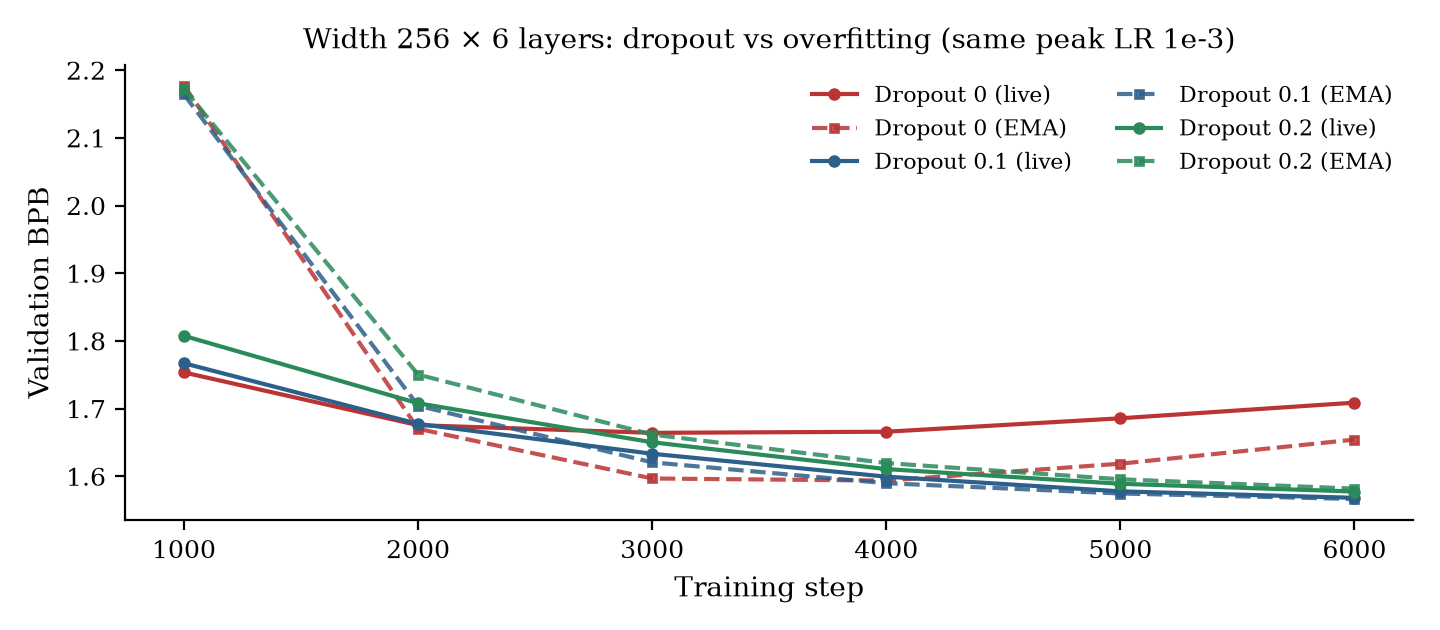
\includegraphics[width=\linewidth]{fig2_dropout_curves.png}
\caption{Width $256\times 6$ layers: dropout versus overfitting at peak LR $10^{-3}$. Solid: live weights; dashed: EMA.}
\label{fig:dropout}
\end{figure}

\section{Final-scale ablation and the SwiGLU reversal}
\label{sec:final}

At the \emph{submitted token budget} ($229$M targets, batch $128$, LR $4\times 10^{-3}$, EMA $0.9995$, dropout $0.2$, seed 17), mechanisms were removed one at a time (Figure~\ref{fig:final}, right). Table~\ref{tab:final} reports EMA validation BPB unless noted.

\begin{table}[t]
\centering
\caption{Final-scale paired ablations ($229$M targets, seed 17).}
\label{tab:final}
\small
\begin{tabular}{lrr}
\toprule
Variant & Val.\ BPB & vs SwiGLU run \\
\midrule
SwiGLU, wd $0.1$ (previous freeze) & 1.4870 & $0$ \\
Same run, \textbf{no EMA} (live weights) & 1.5036 & $+0.017$ \\
RoPE $\to$ learned positions & 1.5311 & $+0.044$ \\
Entire block $\to$ scaled classroom GPT & 1.5153 & $+0.028$ \\
Dropout $0$ & 2.214 (live 2.985) & $+0.73$ \\
\textbf{SwiGLU $\to$ GELU}, wd $0.1$ & \textbf{1.4779} & $-0.009$ \\
GELU, \textbf{wd $0.3$} (submitted) & \textbf{1.4672} & $-0.020$ \\
\bottomrule
\end{tabular}
\end{table}

\begin{figure}[t]
\centering
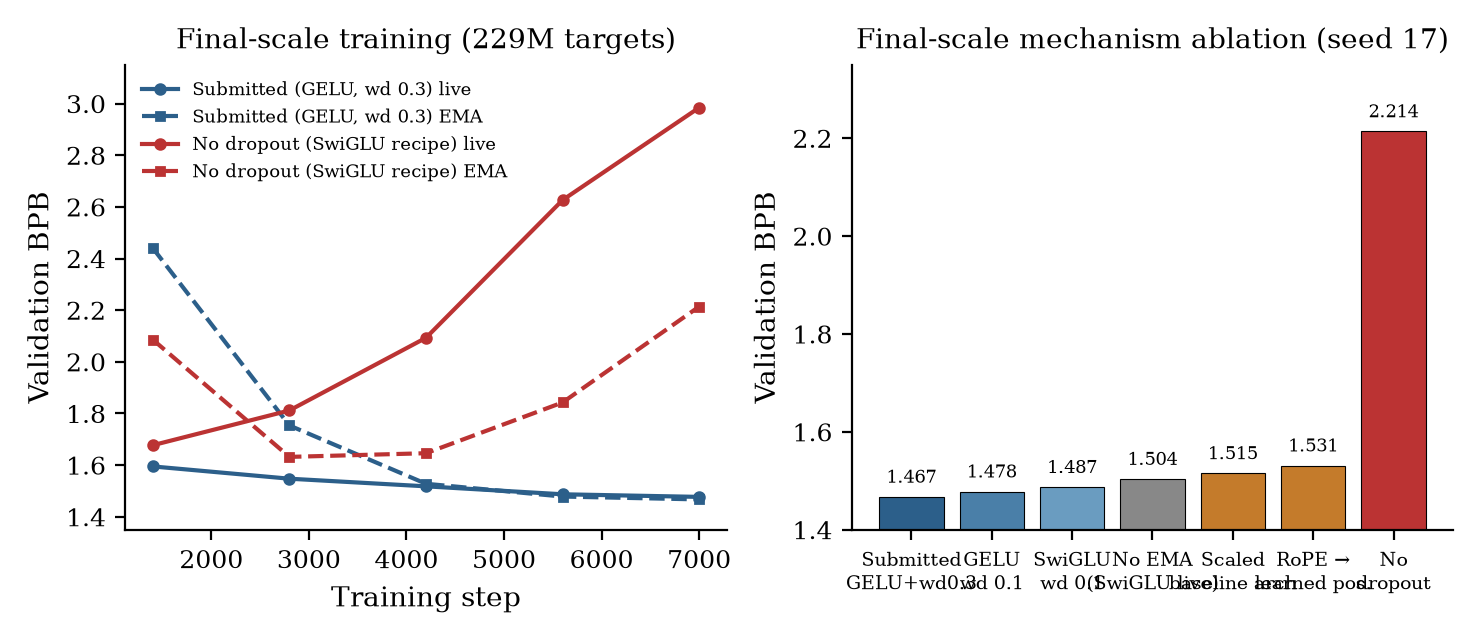
\includegraphics[width=\linewidth]{fig3_final_scale.png}
\caption{Left: live versus EMA validation BPB for the submitted recipe and a no-dropout control. Right: final-scale mechanism ablations (seed 17).}
\label{fig:final}
\end{figure}

\textbf{Dropout} is the dominant regulariser: without it the live model diverges after $\approx 1.4$k steps (Figure~\ref{fig:final}, left). \textbf{EMA} is a cheap averaging of the optimisation path and is worth $\approx 0.01$--$0.017$ BPB at this scale; it is a training-time copy, not a test-time ensemble, so scoring cost is unchanged. \textbf{RoPE} remains helpful but the gain shrinks from $0.16$ (short training) to $0.04$ (long training): more epochs let a learned table catch up, yet not completely. Replacing the whole modern block by a scaled classroom GPT, trained with the \emph{same} recipe, lands at $1.515$: most of the journey from $2.07$ to $1.47$ is \textbf{scale + schedule + dropout + EMA}.

\textbf{SwiGLU reverses sign.} At $9.83$M tokens SwiGLU won by $0.09$; at $229$M tokens with dropout $0.2$, GELU wins by $\approx 0.014$ on average over three seeds (GELU $1.4765\pm 0.0026$ vs SwiGLU $1.4904\pm 0.0036$). A gated MLP is a higher-capacity FFN; once the model is large and the data are seen $\approx 60$ times, that extra capacity overfits even with dropout.

GELU + weight decay $0.3$ is the submitted method. It does not change scoring time relative to a SwiGLU $256\times 8$ checkpoint. CPU scoring of the submitted predictor is about $3.4$--$4.1\times$ the local baseline (quieter host $\approx 3.4\times$), peak RSS is $2.10$\,GiB, and the uncompressed checkpoint is $26.0$\,MiB, all inside the evaluation caps.

\section{Training and search cost}

Development used one RTX 3080~Ti (12\,GiB). About \textbf{68} recorded GPU training runs sum to \textbf{$29\,800$\,s $\approx 8.3$ GPU-hours} of job time (many overlapped on one GPU, so wall-clock was shorter). Additional CPU time: the official 1\,200-step baseline ($\approx 7$\,min), repeated scorer timings, and all ranked FP32 evaluations. No external text, no pretrained weights, no paid API.

\section{Critical analysis}

\paragraph{What worked.}
(i)~RoPE is the one architectural change that helped at \emph{both} token budgets.
(ii)~Dropout plus a long cosine schedule is what makes a $6.8$M model viable on $3.6$M tokens.
(iii)~EMA is a one-line, zero-inference-cost improvement that should be in any ablation table because the trainer already holds the live weights.
(iv)~GELU + stronger weight decay beat a fashionable gated MLP once training was long---an empirical correction, not a slogan.

\paragraph{What did not.}
RMSNorm and dropping bias did not matter at $1$M parameters and were not re-litigated as ``wins.'' Extra heads, extra width at fixed time, and simply training longer without more decay all failed. A 9-layer net used more of the $5\times$ budget for no validation gain: \textbf{the bottleneck is data, not FLOPs.}

\paragraph{Trade-off.}
Moving from the $1.05$M modern GPT (val.\ $1.84$) to the $6.8$M submitted model (val.\ $1.47$) costs about $3\times$ scoring time and $6\times$ parameters, still inside the cap. Further scale would spend the remaining $1\times$ time for a likely sub-$0.01$ BPB and a higher overfitting risk.

\paragraph{Limitations.}
Several late ablations used a single seed; the GELU and weight-decay conclusions were replicated on seeds 18 and 19. The CPU time ratio is host-load dependent; the architecture ratio measured on a quieter interval is $\approx 3.4\times$. Substantive implementation and drafting help from a coding agent (Cursor Grok~4.6) is disclosed in the repository README.

\section{Conclusion}

The submitted predictor is a 256-wide, 8-layer causal GPT with RMSNorm, RoPE, GELU, dropout $0.2$, and EMA weights, trained for $229$M targets with AdamW weight decay $0.3$. It scores \textbf{1.48544} full-test FP32 BPB against a reproduced baseline of \textbf{2.10126}, within the three evaluation limits. The matched-token study isolates RoPE and (under short training) SwiGLU; the final-scale study shows that \textbf{regularisation and training length dominate architecture}, and that SwiGLU \emph{hurts} once the model is large. Those two controls together satisfy the guide's evidence requirement.

\begin{thebibliography}{8}
\bibitem{gpt2}
A.~Radford et al., \emph{Language Models are Unsupervised Multitask Learners}, OpenAI, 2019.

\bibitem{rope}
J.~Su et al., RoFormer: Enhanced Transformer with Rotary Position Embedding, \emph{Neurocomputing} / arXiv:2104.09864.

\bibitem{rmsnorm}
B.~Zhang and R.~Sennrich, Root Mean Square Layer Normalization, \emph{NeurIPS}, 2019.

\bibitem{swiglu}
N.~Shazeer, GLU Variants Improve Transformer, arXiv:2002.05202, 2020.

\bibitem{adamw}
I.~Loshchilov and F.~Hutter, Decoupled Weight Decay Regularization, \emph{ICLR}, 2019.

\bibitem{wikitext}
S.~Merity et al., Pointer Sentinel Mixture Models, \emph{ICLR}, 2017.

\end{thebibliography}

\end{document}
